% !TEX options=--shell-escape
% Beamer template by Julian Lueken

\documentclass[8pt, aspectratio=169]{beamer}
\usepackage[main=ngerman]{babel}
\usepackage[T1]{fontenc}
\usepackage{tikz}
\usepackage{helvet}
\usepackage{lipsum}
\usepackage{float}
\usepackage{svg}
\usepackage{subcaption}
\renewcommand{\familydefault}{\sfdefault}

\definecolor{mypres}{RGB}{97,107,104}

\makeatletter
\newcommand*\bigcdot{\mathpalette\bigcdot@{.5}}
\newcommand*\bigcdot@[2]{\mathbin{\vcenter{\hbox{\scalebox{#2}{$\m@th#1\bullet$}}}}}
\makeatother

% setting some colors for the theme
\setbeamercolor{palette primary}{fg=mypres,bg=white}
\setbeamercolor{palette secondary}{fg=mypres,bg=white}
\setbeamercolor{structure}{fg=mypres,bg=white}
\setbeamercolor{title in head/foot}{fg=black,bg=white}
\setbeamercolor{date in head/foot}{fg=gray,bg=white}

% definition of the headline template
\defbeamertemplate*{headline}{mytheme}{%
	\begin{tikzpicture}[remember picture, overlay]
		\node[text=mypres,anchor=west,font=\sffamily\tiny,text width=0.8\paperwidth] at ([xshift=7pt,yshift=0.5\textheight]current page.west) (header0) {DLR.de{ }$\bigcdot${ }Folie \insertframenumber};
		\node[text=mypres,anchor=west,font=\sffamily\tiny,text width=0.8\paperwidth] at ([xshift=55pt,yshift=0.5\textheight]current page.west) (header1) {$\bigcdot${ }\insertshorttitle{ }$\bigcdot${ }\insertauthor{ }$\bigcdot${ }\insertdate};
	\end{tikzpicture}
	\vskip15pt
}

% definition of the footline template arial
\defbeamertemplate*{footline}{mytheme}{%
	\begin{tikzpicture}[remember picture, overlay]
		\node[inner sep=0, anchor = south east] at (current page.south east) (banner) {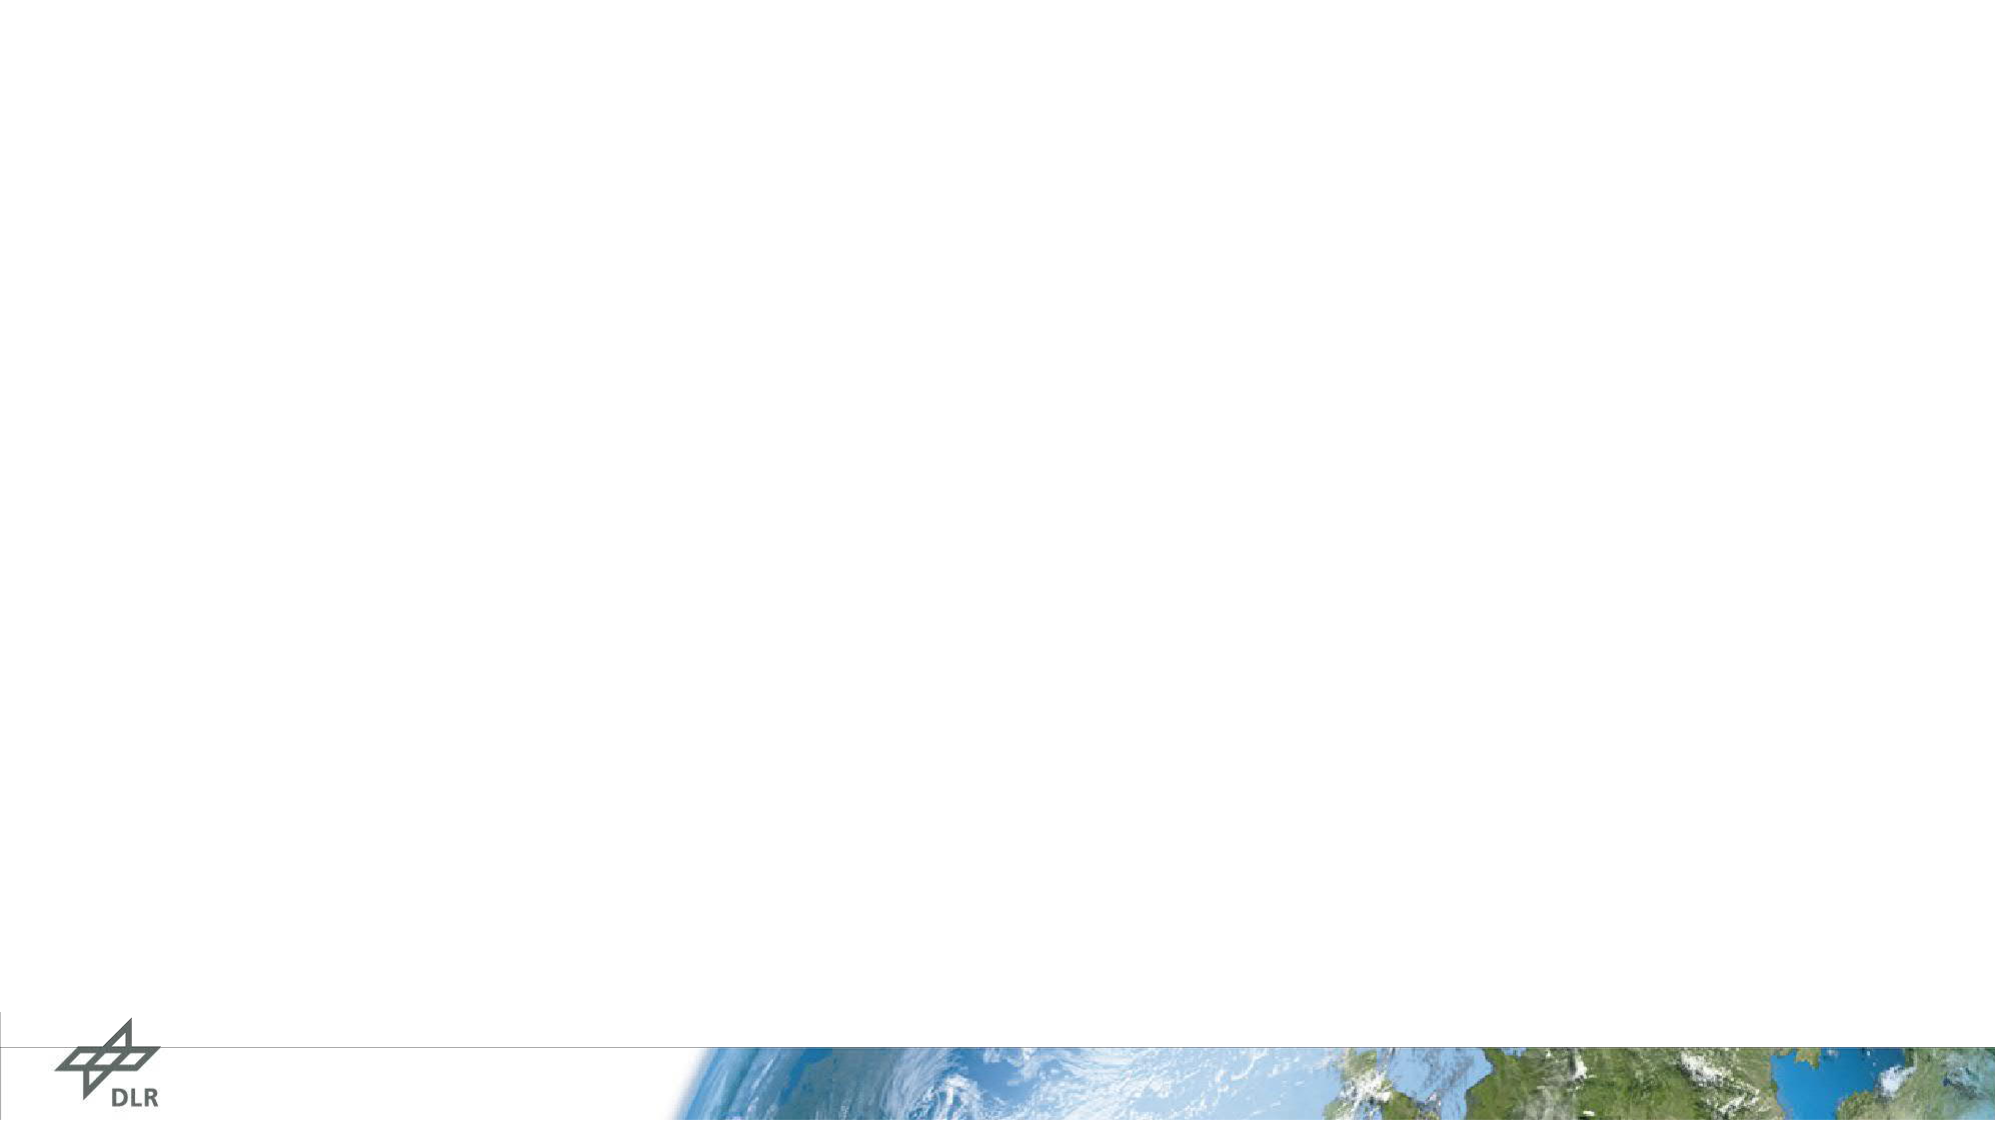
\includegraphics[page=1, width=\paperwidth]{footer.pdf}};
	\end{tikzpicture}
	\vskip0pt
}

% definition of the title page template
\defbeamertemplate*{title page}{mytheme}[1][] {
	\begin{tikzpicture}[remember picture, overlay]
		\node[text=mypres,anchor=west,font=\sffamily\tiny,text width=0.8\paperwidth] at ([xshift=6pt,yshift=0.5\textheight]current page.west) (header0) {DLR.de{ }$\bigcdot${ }Folie \insertframenumber};
		\node[text=mypres,anchor=west,font=\sffamily\tiny,text width=0.8\paperwidth] at ([xshift=54pt,yshift=0.5\textheight]current page.west) (header1) {$\bigcdot${ }\insertshorttitle{ }$\bigcdot${ }\insertauthor{ }$\bigcdot${ }\insertdate};
		\node[inner sep=0, anchor = south east] at (current page.south east) (banner) {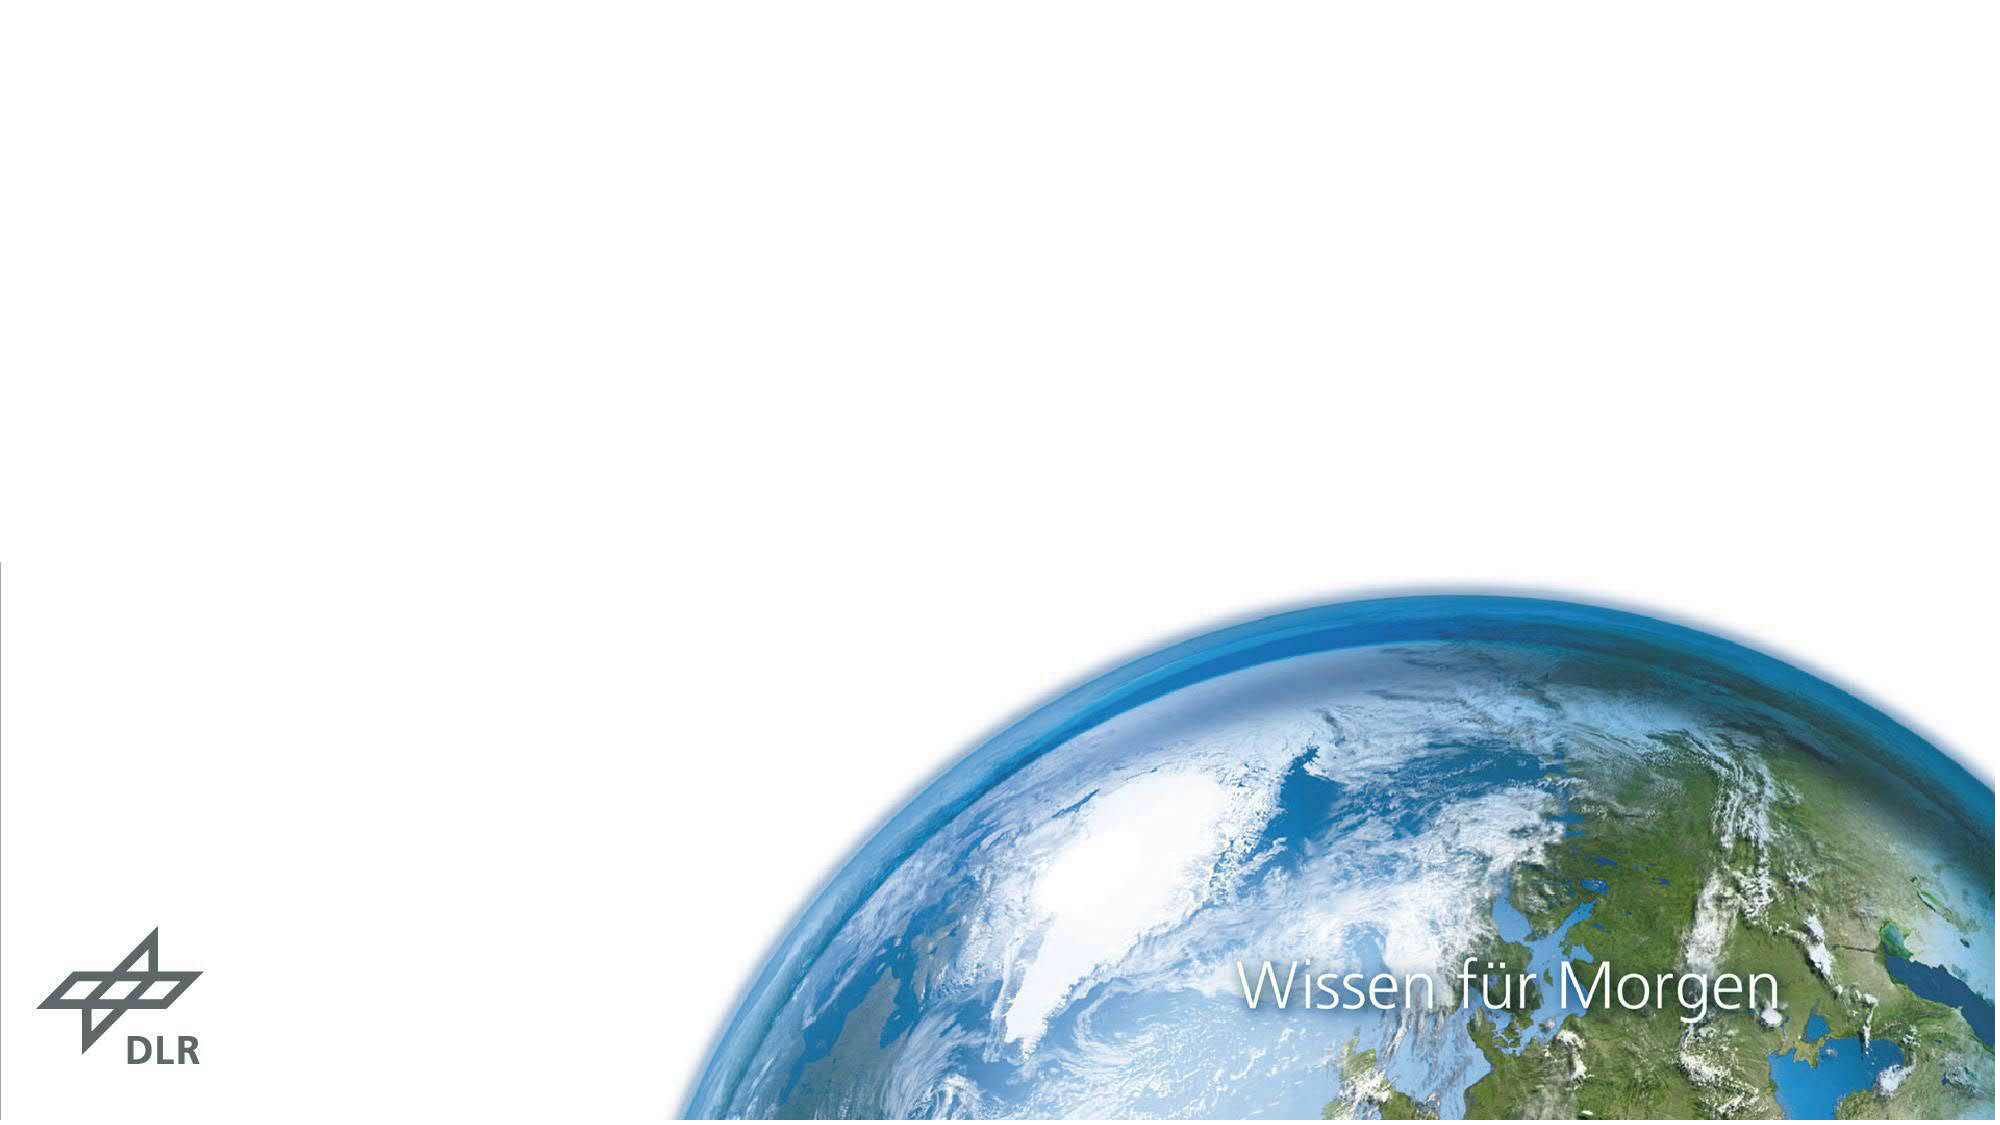
\includegraphics[page=1, width=\paperwidth]{header.pdf}};
		\node[text=mypres,anchor=south west,font=\sffamily\LARGE,text width=0.8\paperwidth] at ([xshift=7pt,yshift=1.50cm]current page.west) (title) {\raggedleft\insertshorttitle};
		\node[text=mypres,anchor=south west,font=\sffamily\large,text width=0.8\paperwidth] at ([xshift=7pt,yshift=1.00cm]current page.west) (subtitle) {\raggedleft\inserttitle};
		\node[text=mypres,anchor=south west,font=\sffamily,text width=.55\paperwidth] at ([xshift=7pt,yshift=-1cm]current page.west) (author) {\raggedright\insertauthor};
		\node[text=mypres,anchor=south west,font=\sffamily,text width=.55\paperwidth] at ([xshift=7pt,yshift=-1.5cm]current page.west) (date) {\raggedright\insertdate};
	\end{tikzpicture}
	\vskip0pt
}

% remove navigation symbols
\setbeamertemplate{navigation symbols}{}

\title[CoolingGen]{Eine Software zur Erstellung von Kühlungsgeometrien}
\author{Julian Lüken}
\date{\today}

\begin{document}

\begin{frame}[plain]
	\maketitle
\end{frame}

\begin{frame}
	\frametitle{Inhalt}
	\vspace{-1cm}\hspace{-0.5cm}
	\begin{minipage}[t]{\textwidth}
		\begin{itemize}
			\item Einleitung
			\item Motivation
			\item Ergebnisse
			\item Methoden
			\item Fragen
		\end{itemize}
	\end{minipage}
	\vfill
\end{frame}

\begin{frame}
	\frametitle{Einleitung/Motivation}
	\vspace{-1cm}\hspace{-0.5cm}
	\begin{minipage}[t]{\textwidth}
		Was ist CoolingGen?
		\begin{itemize}
			\item Programm, welches mithilfe von CAD eine Schaufel aus BladeGen mit Kühlungsgeometrien ausstattet
			\item Basiert auf BasicTools (Bibiliothek vom DLR für B-Spline Kurven/Flächen)
			\item Entwicklung startete 2013 (Autoren: C. Voß, T. Schu...)
			\item Meine Arbeit daran startete im Juli 2021
		\end{itemize}
		\vspace{0.5cm}
		Warum CoolingGen?
		\begin{itemize}
			\item Erzeugung von Kühlungsgeometrien innerhalb einer Schaufel mit herkömmlichen CAD-Tools ist mühsam und dauert lange
			\item Laufzeit von CoolingGen: ca. 20 Sekunden auf 8 $\cdot$ 3GHz
			\item Ermöglicht Optimierung von Kühlungsgeometrien durch Phasenraumsuche gekoppelt mit CFD-Simulationen
		\end{itemize}

	\end{minipage}
	\vfill
\end{frame}

\begin{frame}
	\frametitle{Einleitung/Motivation}
	\vspace{-1cm}\hspace{-0.5cm}
	\begin{minipage}[t]{\textwidth}
		Input:
		\begin{itemize}
			\item Schaufelgeometrie aus BladeGen
			\item Parameter für die Kühlungsgeometrien (als XML)
		\end{itemize}
		Output:
		\begin{itemize}
			\item Kühlungsgeometrien (als STEP, für CENTAUR und für Tecplot)
		\end{itemize}

		Welche Geometrien kann CoolingGen erzeugen?
		Derzeit unterstützt (und hier vorgestellt):
		\begin{itemize}
			\item Kühlkanäle (mit Umkehrungen)
			\item Prallbleche (mit Bohrungen)
			\item Filmkühlung
		\end{itemize}

		To-do:
		\begin{itemize}
			\item Ausblasungsschlitze
			\item Pin-fins (Kühlrippen)
		\end{itemize}
	\end{minipage}
	\vfill
\end{frame}

\begin{frame}
	\frametitle{Ergebnisse}
	\vspace{-1cm}\hspace{-0.5cm}
	\begin{minipage}[t]{.69\textwidth}
		\centering
		<Kanal mit Umlenkungen und FK Bohrungen>
	\end{minipage}
	\begin{minipage}[t]{.29\textwidth}
		\centering
		<Kanal mit Impingement Inserts>
	\end{minipage}
	\vfill
\end{frame}

\begin{frame}
	\frametitle{Methoden}
	\vspace{-1cm}\hspace{-0.5cm}
	\begin{minipage}[t]{\textwidth}
		\begin{center}
		Größte Herausforderung? Robuste und performante Verschnittalgorithmen!
		\end{center}
		\vspace{0.5cm}
		\begin{center}
		\emph{The single greatest cause of poor reliability of CAD systems is lack of topologically consistent surface intersection algorithms.}
		\end{center}
		\vspace{0.5cm}
		\flushright -- \emph{Closing the Gap Between CAD Model and Downstream Applications} by R. Farouki
	\end{minipage}
\end{frame}

\begin{frame}
	\frametitle{Methoden / Kanäle und Prallbleche}
	\vspace{-1cm}\hspace{-0.5cm}
	\begin{minipage}[t]{\textwidth}
		Um die Kanäle zu erzeugen, müssen (neben anderen Parametern) die Kanalwände als Input spezifiziert werden
		wird folgende Strategie verwendet:
		\begin{enumerate}
			\item Schaufeloberfläche in radialer Höhe $n$ mal gesamplet $\rightarrow$ erhalten $n$ Profilkurven
			\item Koordinatentransformation $(x, y, z) \rightarrow (x, r) \rightarrow (m', \theta)$
			\item Unterteilung der Profilkurven an den Kanalwänden
			\item \emph{Schrumpfen} der Profilkurven (abhängig von Saug-/Druck-/Wandseite)
			\item Einpassung von \emph{Fillets} an \emph{Knicken/Ecken}
			\item Rücktransformation nach $(x, y, z)$, und \emph{Lifting}
		\end{enumerate}
	\end{minipage}
	\vfill
\end{frame}

\begin{frame}
	\frametitle{Methoden / Kanäle und Prallbleche / Unterteilung}
	\vspace{-1cm}\hspace{-0.5cm}
	\begin{minipage}[t]{.3\textwidth}
		Unterteilung der Profilkurve mithilfe von \emph{Ray-Marching}.
	\end{minipage}
	\begin{minipage}{.68\textwidth}
		\begin{figure}[H]
			\centering
			\includesvg[width=\textwidth]{../python/rayMarching}
		\end{figure}
	\end{minipage}
\end{frame}

\begin{frame}
	\frametitle{Methoden / Kanäle und Prallbleche / Unterteilung}
	\vspace{-1cm}\hspace{-0.5cm}
	\begin{minipage}[t]{.69\textwidth}
		\centering
		<Bild von Profilkurve mit Skelettlinie und Wänden>
	\end{minipage}
	\begin{minipage}[t]{.29\textwidth}
		\centering
		<Bild von Kammerschnitt>
	\end{minipage}
\end{frame}

\begin{frame}
	\frametitle{Methoden / Kanäle und Prallbleche / Schrumpfen}
	\vspace{-1cm}\hspace{-0.5cm}
	\begin{minipage}[t]{\textwidth}
		Schrumpfen erfordert die Detektion von Selbst-Schnittpunkten, aber auch dieser Prozess hinterlässt \emph{Knicke}.
		Der Fachbegriff für solche Kurven, der auch in herkömmlicher CAD Software zu finden ist, lautet \emph{Offset-Kurve}.
	\end{minipage}
	\begin{figure}[H]
		\centering
		\begin{subfigure}{0.49\textwidth}
			\includesvg[width=0.98\textwidth]{../python/offsetCurveSelfIntersection0}
		\end{subfigure}
		\begin{subfigure}{0.49\textwidth}
			\includesvg[width=0.98\textwidth]{../python/offsetCurveSelfIntersection1}
		\end{subfigure}
	\end{figure}
\end{frame}

\begin{frame}
	\frametitle{Methoden / Kanäle und Prallbleche / Schrumpfen}
	\vspace{-1cm}\hspace{-0.5cm}
	\begin{minipage}[t]{.32\textwidth}
		\centering
		<Geschrumpft/Fishtails>
	\end{minipage}
	\begin{minipage}[t]{.32\textwidth}
		\centering
		<Geschrumpft/Getrimmt>
	\end{minipage}
	\begin{minipage}[t]{.32\textwidth}
		\centering
		<Geschrumpft/Getrimmt/Fillets>
	\end{minipage}
\end{frame}

\begin{frame}
	\frametitle{Methoden / Kanäle und Prallbleche / Fillets}
	\vspace{-1cm}\hspace{-0.5cm}
	\begin{figure}[H]
		\centering
		\includesvg[width=\textwidth]{../python/filletConstruction1}
		\label{fig:filletconstruction}
	\end{figure}
	\begin{figure}[H]
		\centering
		\includesvg[width=\textwidth]{../python/filletConstruction2}
	\end{figure}
\end{frame}

\begin{frame}
	\frametitle{Methoden / Kanäle und Prallbleche / Fillets}
	\vspace{-1cm}\hspace{-0.5cm}
	\begin{minipage}[t]{.49\textwidth}
		\centering
		<Bild von Kammerschnitt o Fillets>
	\end{minipage}
	\begin{minipage}[t]{.49\textwidth}
		\centering
		<Bild von Kammerschnitt m Fillets>
	\end{minipage}
\end{frame}

\begin{frame}
	\frametitle{Methoden / Kanäle und Prallbleche / Lifting}
	\vspace{-1cm}\hspace{-0.5cm}
	\begin{minipage}[t]{.49\textwidth}
		\centering
		<Bild von Kammerschnitten>
	\end{minipage}
	\begin{minipage}[t]{.49\textwidth}
		\centering
		<Bild von Kammern>
	\end{minipage}
\end{frame}

\begin{frame}
	\frametitle{Methoden / Umkehrungen}
	\vspace{-1cm}\hspace{-0.5cm}
	\begin{minipage}[t]{\textwidth}
		Strategie:
		\begin{enumerate}
			\item Berechnung einer Kombination aus den zwei Kanälen, die sich zur Umkehrung verbinden
			\item Schneiden der kombinierten Kanäle mit $n$ Ebenen $\rightarrow$ $n$ planare Profilkurven
			\item Verformen der $n$ Kurven
			\item Lifting
		\end{enumerate}
	\end{minipage}
\end{frame}

\begin{frame}
	\frametitle{Methoden / Umkehrungen}
	\vspace{-1cm}\hspace{-0.5cm}
	\begin{minipage}[t]{.49\textwidth}
		\centering
		<Bild aus Gitlab>
	\end{minipage}
	\begin{minipage}[t]{.49\textwidth}
		\centering
		<Bild einer Turnfläche>
	\end{minipage}
\end{frame}

\begin{frame}
	\frametitle{Methoden / Bohrungen}
	\vspace{-1cm}\hspace{-0.5cm}
	\begin{minipage}[t]{.49\textwidth}
		\centering
		<Schema der Kurven einer FK Bohrung>
	\end{minipage}
	\begin{minipage}[t]{.49\textwidth}
		\centering
		<Bild von Robin von Bohrung mit Params>
	\end{minipage}
\end{frame}

\begin{frame}
	\frametitle{Methoden / Fazit}
	\vspace{-1cm}\hspace{-0.5cm}
	\begin{minipage}[t]{.49\textwidth}
		\centering
		Man braucht robuste, schnelle Verschneidungsalgorithmen, und einer reicht nicht:
		\begin{enumerate}
			\item Punkt/Kurve (um den passenden Parameter auf der Kurve zu finden)
			\item Ray/Kurve
			\item Kurve/Kurve und Kurve mit sich selbst
			\item Fläche/Ebene
			\item Fläche/Kurve
		\end{enumerate}
		Überdies wird eine bestimmte Gestalt dieser Schnitte angenommen, um die Algorithmen effizient zu gestalten. Beispielsweise wird bei Kurve/Kurve die Annahme getroffen, dass sich diese beiden nur an einer endlichen Vereinigung von einelementigen Punktmengen treffen. Das ist zwar ausreichend, aber nicht der allgemeine Fall. Für den allgemeinen Fall gibt es gar keine "richtige" Lösung.
	\end{minipage}
\end{frame}

\begin{frame}
	\frametitle{Methoden / Umkehrungen}
	\vspace{-1cm}\hspace{-0.5cm}
	\begin{minipage}[t]{.49\textwidth}
		\centering
		<Bild aus Gitlab>
	\end{minipage}
	\begin{minipage}[t]{.49\textwidth}
		\centering
		<Bild einer Turnfläche>
	\end{minipage}
\end{frame}

\begin{frame}
	\frametitle{Recap}
	\begin{minipage}[t]{\textwidth}
		\centering
		Kopie der Folie mit den Ergebnissen
	\end{minipage}
\end{frame}

\begin{frame}
	\frametitle{}
	\begin{minipage}[t]{\textwidth}
		\centering
		\Large Fragen/Anmerkungen?
	\end{minipage}
\end{frame}

\end{document}